\section{Criação de Componente customizado}

Nesta seção veremos como criar um campo customizado em uma tela. Iremos partir
do modelo de \texttt{CRUD} gerado automaticamente pelo \texttt{MDArte}, para a
entidade \texttt{Estudante}, e faremos as alterações necessárias para a criação
de um novo componente. O componente a ser desenvolvido, somente a título de
exemplo, será um campo texto com máscara para \texttt{CPF}.

Podemos ver o estado inicial do modelo na imagem \ref{modelo_consulta_estudante_custom}.

\begin{figure}[H]
	\centering
	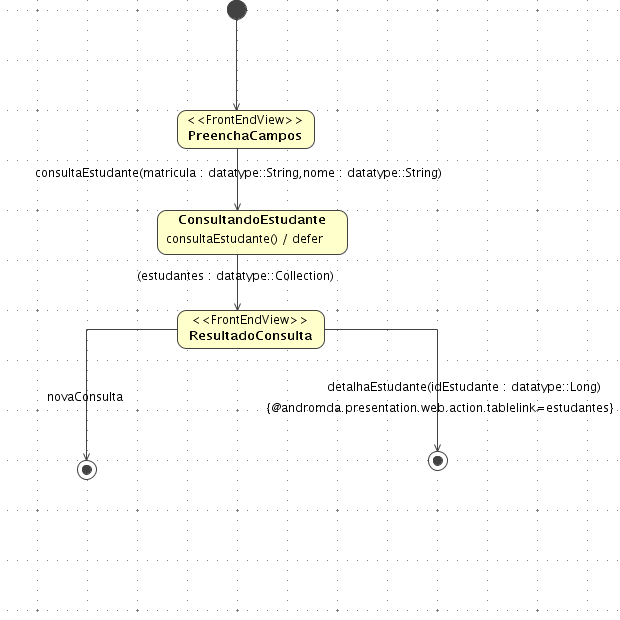
\includegraphics[width=350pt,height=300pt]{files/imgs/tutorial-mdarte-0028.png}
	\caption{Modelo do caso de uso Consulta Estudante.}
	\label{modelo_consulta_estudante_custom}
\end{figure}

Abriremos então a especificação da \texttt{transition}
\texttt{'consultaEstudante'}, clicaremos no botão \texttt{'edit'}, no
\texttt{fieldset} \texttt{'trigger'}, selecionaremos então a aba
\texttt{'parameters'}, da janela aberta quando clicamos o botão anterior, e
clicaremos então no botão \texttt{add}.

Preencheremos então os dados do campo conforme a imagem
\ref{dados_campo_custom_cpf}, SEM, no entanto, clicar no botão \texttt{Ok}.

\begin{figure}[H]
	\centering
	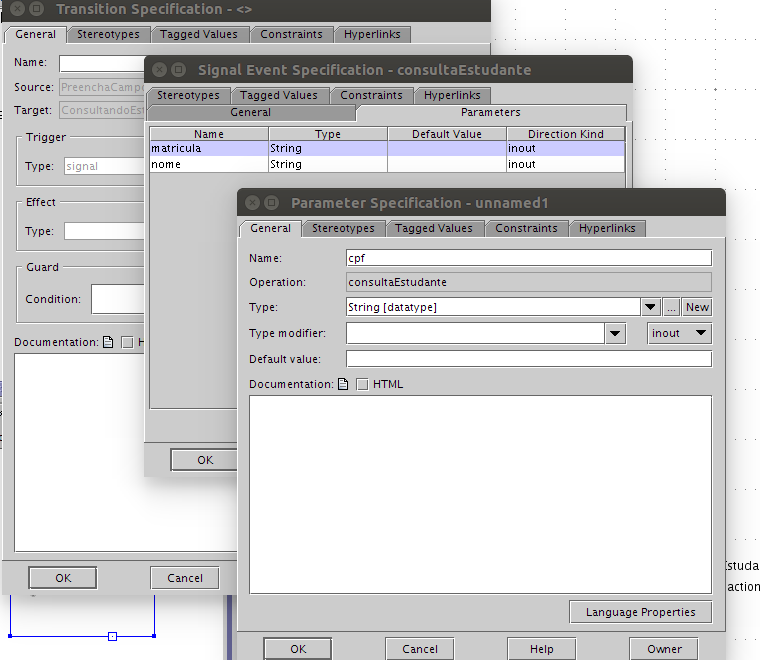
\includegraphics[width=350pt,height=300pt]{files/imgs/tutorial-mdarte-0033.png}
	\caption{Dados do campo 'cpf'.}
	\label{dados_campo_custom_cpf}
\end{figure}

Ainda na mesma janela, selecionaremos a aba \texttt{tagged values},
selecionaremos o \texttt{tagged value} 
\texttt{@andromda.presentation.web.view.field.type}, clicaremos no botão
\texttt{create value} e selecionaremos a opção \texttt{'custom'}, no campo
\texttt{combobox} que será exibido, como na imagem \ref{parametro_cpf_custom}.

\begin{figure}[H]
	\centering
	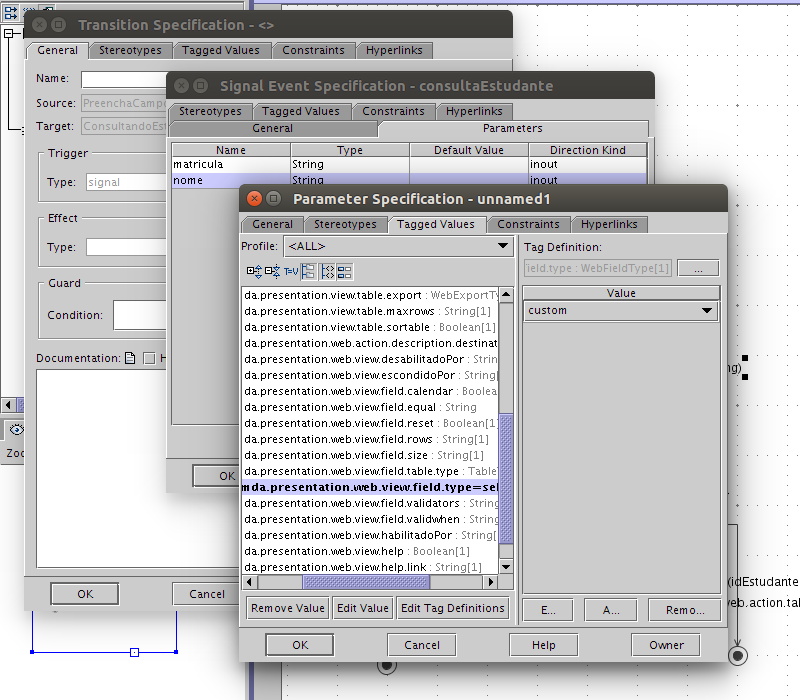
\includegraphics[width=350pt,height=300pt]{files/imgs/tutorial-mdarte-0034.png}
	\caption{Selecionando tipo custom para o campo 'cpf'.}
	\label{parametro_cpf_custom}
\end{figure}

Salvaremos então o modelo e digitaremos os seguintes comandos para regerar o
modelo:

\begin{lstlisting}[language=bash, frame=single, breaklines=true]
maven mda -Dprojeto=sistemaaacademico-geral-Estudante
\end{lstlisting}

Feito isto, o \texttt{MDArte} gerará um arquivo no padrão
\texttt{<nome-do-campo>.jsp}, neste caso, \texttt{cpf.jsp}, no caminho
\texttt{<nome-sistema>/web/<modulo-web>/src/jsp/<caminho-do-pacote-base>/web/<modulo-web>/<nome-caso-de-uso>},
mas você também pode encontrá-lo, no eclipse, através do comando
\texttt{ctrl+shift+r}, digitando o nome do arquivo na janela que é aberta por
esse comando.

Aberto o arquivo, adicionaremos a este o seguinte código \texttt{jsp}:

\lstinputlisting[language=html, frame=single, breaklines=true]{files/jsp/cpf.jsp}

O \texttt{html} adicionado será importado para a tela do sistema no espaço do
formulário dedicado ao campo \texttt{cpf}.

Adicionado o \texttt{jsp} do nosso componente, uma vez que se trata de um campo
de texto com um determinado comportamento (formatar a entrada no modelo do CPF),
precisamos agora adicionar um mecanismo de controle para o comportamento do
campo. Para tal, utilizaremos o \texttt{framework} para \texttt{javascript}
JQuery, uma vez que este já vem com o \texttt{MDArte}, além do fato de o
\texttt{JQuery} já possuir uma funcionalidade nativa que faça isso.

Para adicionar código \texttt{Javascript} manualmente a uma \texttt{view}
precisamos abrir o arquivo \texttt{<nome-da-view>-impl.js}, no mesmo caminho
do arquivo \texttt{jsp} alterado acima. O arquivo alterado é destinado ao código
adicionado pelo desenvolvedor para customizar o comportamento da aplicação, não
sendo sobrescrito durante a geração. Certifique-se, portanto, de estar
adicionando o seu código nestes pontos de implementação, a fim de não perdê-lo
na próxima geração.

Adicionaremos agora o seguinte código \texttt{JavaScript} ao arquivo
\texttt{preencha-campos-impl.js}:

\lstinputlisting[language=c, frame=single, breaklines=true]{files/js/preencha-campos-impl.js}

Executaremos agora o seguinte comando para compilar e dar \texttt{deploy} no
projeto:
\begin{lstlisting}[language=bash, frame=single, breaklines=true]
maven compile deploy
\end{lstlisting}

Abrindo o sistema e acessando a \texttt{view} \texttt{'Preencha Campos'} do caso
de uso \texttt{Consulta Estudante}, podemos conferir o resultado do nosso
componente \texttt{custom} de nome \texttt{cpf}, como na imagem
\ref{parametro_cpf_custom_exemplo}.
\begin{figure}[H]
	\centering
	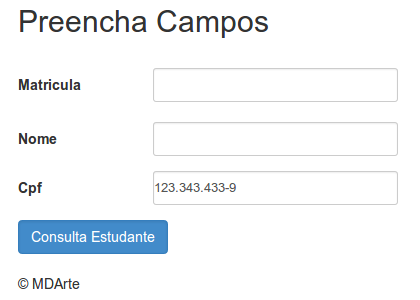
\includegraphics[width=280pt,height=200pt]{files/imgs/tutorial-mdarte-0035.png}
	\caption{Resultado de componente custom de nome 'cpf'.}
	\label{parametro_cpf_custom_exemplo}
\end{figure}